\documentclass[a4paper, 12pt, final]{article}

\usepackage{fixme}
%\usepackage{url}
\usepackage{hyperref}
\usepackage{graphicx}
\usepackage{float}
\usepackage{varioref}
\usepackage{boxedminipage}
\hypersetup{colorlinks=true}

\title{
  
\includegraphics[height=1in]{View_World_Logo.jpg}\\
  View World reporting system user manual (draft version)
  }

\author{
  Rune Bech Persson\\
  \url{rbp@viewworld.dk}
}

\date{\today}

\usepackage{fancyhdr}
\renewcommand{\headheight}{0.6in}
\setlength{\headwidth}{\textwidth}
\fancyhead[L]{}% empty left
\fancyhead[R]{ % right
  
\includegraphics[height=0.3in]{View_World_Logo.jpg}
}
\pagestyle{fancy}

\begin{document}

\maketitle

\newpage

\tableofcontents

\newpage

\section{Getting Started}

This manual describes the use of the ViewWorld reporting system.

The reporting system is primarily designed for use by Non Governmental Organisations working in developing countries. This manual is therefore written with these users in mind.

This manual covers the ViewWorld android application, as well as the use of the web-interface on viewworld.dk where data can be viewed, edited and deleted. Also the management of users and forms will be covered.

Before getting started using the View World reporting application a few preparations will have to be made. A phone running android 1.5 or greater must be available. If data should be uploaded via a mobile network, a data enabled sim card is also required.

\section{Android phone}

The android version must be larger than 1.5 to be able to run the ViewWorld reporting system. All new phones ship with android version 1.5 or larger.

There are many manufacturers of Android phones. Some make them cheap with very few features, and some are expensive with a large set of functionality such as high resolution screen, acceleration sensors, HD video recording. However not all of these functions are required when using the View World reporting system. Below is a list of the phone features which are used in the reporting system and which should be considered when buying an android phone.

\begin{description}
\item[Video] A video enabled phone is not a requirement. However the system is capable of saving video clips if a video recorder is available..
\item[Pictures] A camera enabled phone should be used. Almost all android phones have cameras integrated. 
\item[Sound] A sound recorder can be installed in all android phones. If the sound recorder is not installed when trying to record sound, the View World app will guide you to the android market for installation.
\item[GPS] The phone should be GPS enabled. This will allow geo-tagging of reports, and make it easy to visualize reports in a map.
\item[WiFi] If the mobile network is slow, it may be useful to buy WiFi enabled phones. This way, data can be transmitted using a normal WiFi network.
\item[3G] Fast mobile network is required if high quality images or videos are recorded and sent from the field.
\item[Battery] Battery capacity is an important thing to consider when buying a phone. In some cases it can be difficult to charge the phone on the go, so therefore choose a phone with a large battery capacity.
\item[Ruggedness] If the phone is to be used in demanding environments it may be a good idea to buy a rugged phone. Waterproof, dust resistant phones can be bought.
\end{description}

ViewWorld has tested the Motorola Defy Rugged phone and currently recommend this phone for reporting in hard environments. It is water and dust-proof and contains all important features. However if ruggedness is not a requirement, much cheaper phones can be bought. Contact \url{rbp@viewworld.dk} for more information.

\subsection{Network subscription}

The View World reporting system supports two ways of sending and receiving data. 
One method uses a WiFi network which is frequently available in offices, homes and Internet cafe's. Using this method a subscription fee does not apply when sending data, furthermore the data connection is usually very fast.

The other way of sending data is through a mobile network. This allows a field officer to send in reports while he/she is still in the field saving time on travel. To send data from the field, a network subscription is required. When choosing a mobile network operator the following aspects should be considered:

\begin{description}
\item[Speed] The speed of the network is determined by the technology the network operator uses. A 3G network is very fast, while GPRS and EDGE networks are fast but may limit uploading of videos and other large media files. A slower connection may be used, but it is emparative that data/internet subscription is available for the system to function.
\item[Coverage] The network coverage is an important aspect to consider when choosing network operator. A good coverage will allow sending of data from remote areas. Network operators generally have coverage maps on their homepage, and these should be examined before a network operator is chosen.
\end{description}

\fbox{
\emph{IMPORTANT: The network operator must support data transfer}}

\subsection{Installing application}

When data connection is achieved on the Android phone installation is simple. Use Android market to search for ViewWorld and install the View World application. 

If installation via Android Market is not possible, go to \url{viewworld.dk/demo} and click on the download link or use the 2D barcode. The installation of the View World application should now start.

If a you are asked whether to grant access to phone features for the View World app, answer yes to all guestions.

When you have installed the ViewWorld application you can start it by clicking on the icon in the program list as seen in figure \ref{fig:vw_app_icon}.

\begin{figure}[h!]
  \centering
      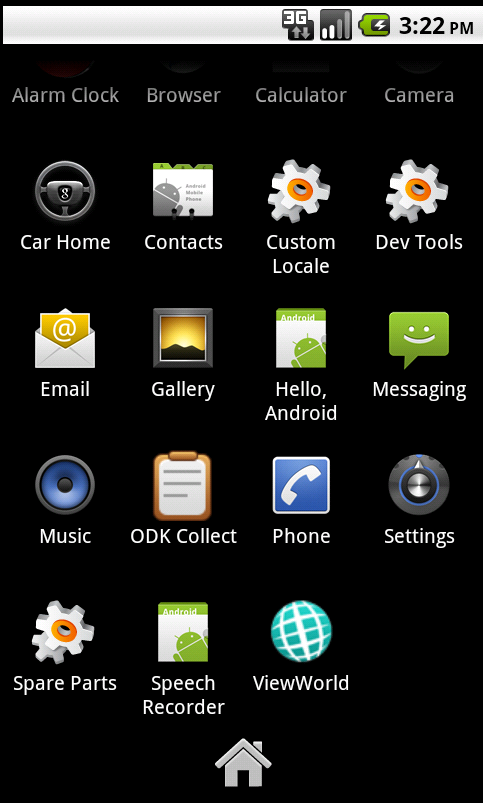
\includegraphics[width=0.35\textwidth]{pics/vw_app_icon.png}
  \caption{Press the ViewWorld logo in the programs list to start the reporting application}
  \label{fig:vw_app_icon}
\end{figure}

\subsection{Setup}

Setting up the application is required to make sure that reports are delivered to the correct organisation database. This requires entering the user name and password given by the organisation using the View World reporting system. You also need to download the forms you wish to use to the phone before you can start reporting. Downloading forms must be done when internet connection is available and should therefore be done before leaving for a field visit.

\subsubsection{Server settings}

When starting the phone for the first time the main menu is shown as in figure \ref{fig:front_screen}.

\begin{figure}[h!]
  \centering
      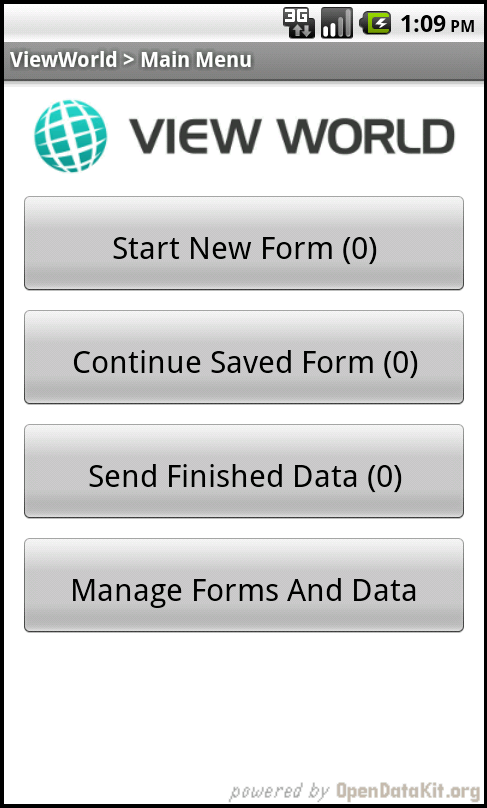
\includegraphics[width=0.35\textwidth]{pics/vw_front_screen.png}
  \caption{The main menu of the View World reporting system}
  \label{fig:front_screen}
\end{figure}

Pressing the \emph{menu} button on the phone opens a settings screen in the bottom of the main menu as seen in figure \ref{fig:server_prefs_1}. Pressing the \emph{server preferences} button opens the settings screen where user name and password can be entered as seen in figure \ref{fig:server_prefs_2}

\begin{figure}[h!]
  \centering
      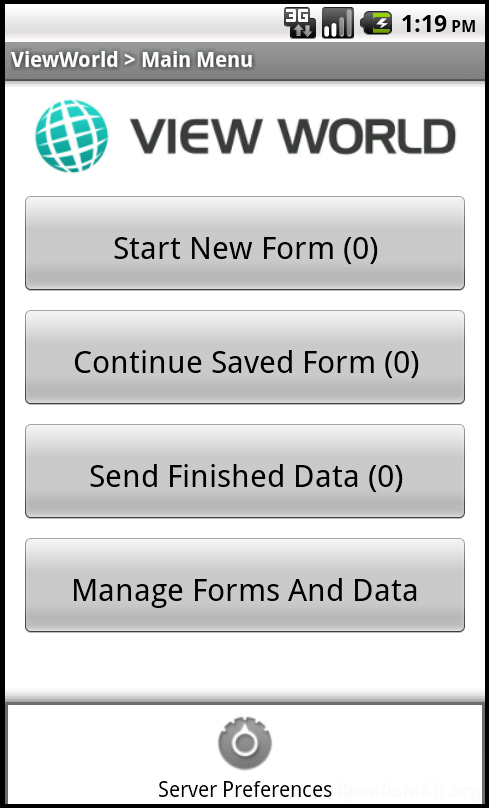
\includegraphics[width=0.35\textwidth]{pics/vw_server_pref_1.png}
  \caption{Clicking on the menu button on the phone gives access to server preferences}
  \label{fig:server_prefs_1}
\end{figure}

\begin{figure}[h!]
  \centering
      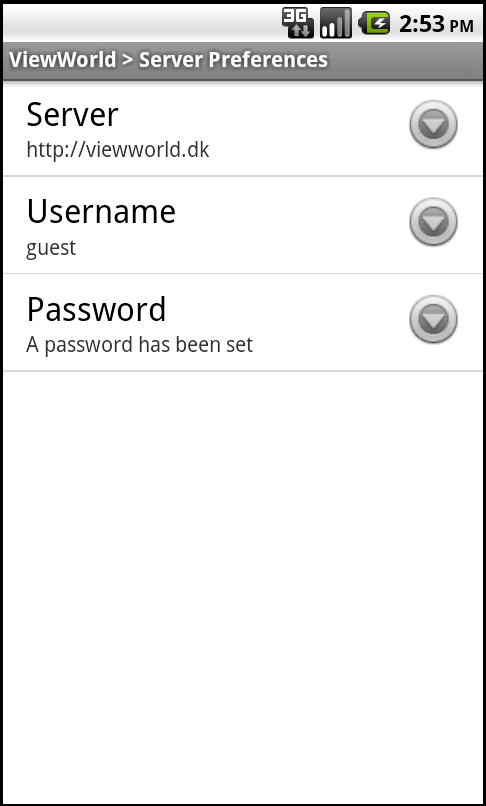
\includegraphics[width=0.35\textwidth]{pics/vw_server_pref_2.png}
  \caption{Enter your username and password. The server must be set to http://viewworld.dk}
  \label{fig:server_prefs_2}
\end{figure}

\subsubsection{Downloading forms}

To get started reporting, you first need to download the forms you wish to use on the phone.

To enter the form management interface click on \emph{manage forms and data} in the main menu. The page shown in figure \ref{fig:manage_forms_and_data} opens and shows the list of forms available on the phone. When starting up the application for the first time, there will be no forms available on the phone and this screen is empty.

\begin{figure}[h!]
  \centering
      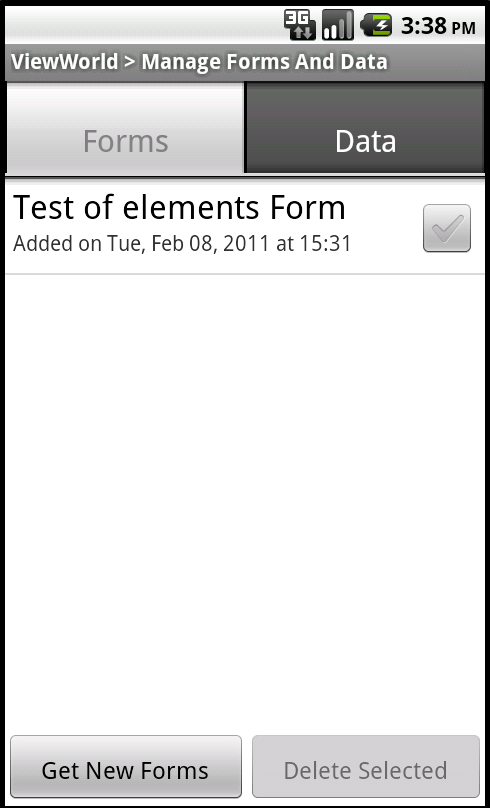
\includegraphics[width=0.35\textwidth]{pics/manage_forms_and_data.png}
  \caption{This shows the forms available on the phone. To download new forms press \emph{Get New Forms}}
  \label{fig:manage_forms_and_data}
\end{figure}

To get new forms click on \emph{Get New Forms}. If the phone is connected to the internet, a list of available forms as seen in figure \ref{fig:get_new_forms} will be shown after a short time. Select the forms you wish to download to the phone, and click on \emph{Get Selected}. The form(s) are downloaded to the phone and are available for reporting and now shows up in the form list as seen in figure \ref{fig:new_form_downloaded}.

\begin{figure}[h!]
  \centering
      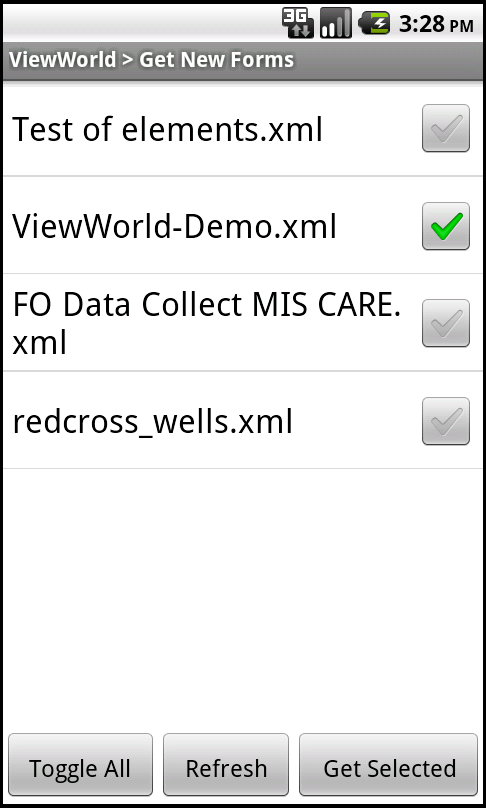
\includegraphics[width=0.35\textwidth]{pics/get_new_forms.png}
  \caption{Select the forms you wish to download to the phone and press \emph{Get Selected}. The forms are downloaded and now available on the phone for reporting.}
  \label{fig:get_new_forms}
\end{figure}

\begin{figure}[h!]
  \centering
      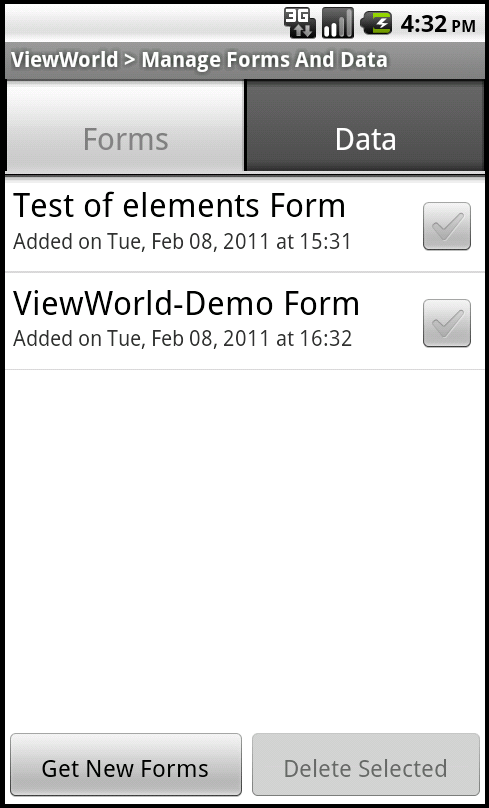
\includegraphics[width=0.35\textwidth]{pics/new_form_downloaded.png}
  \caption{The list of forms now includes the newly downloaded \emph{ViewWorld-Demo} form}
  \label{fig:new_form_downloaded}
\end{figure}

\newpage
\subsection{Basic use}

Here the basic use of the ViewWorld reporting application will be described. This includes starting a new report, how to enter data and how to send data to the server.

\subsubsection{Fill in a report}

To start a new report go to the main menu and press \emph{Start New Report}. The screen in figure \ref{fig:start_new_form_list} appear and shows the list of reports that are available for you to fill in. Pressing one of these takes you to the start screen of the report, which is always a guide to how to move between the different questions. This can be seen in figure \ref{fig:new_report_first_screen}.

\begin{figure}[!htbp]
  \centering
      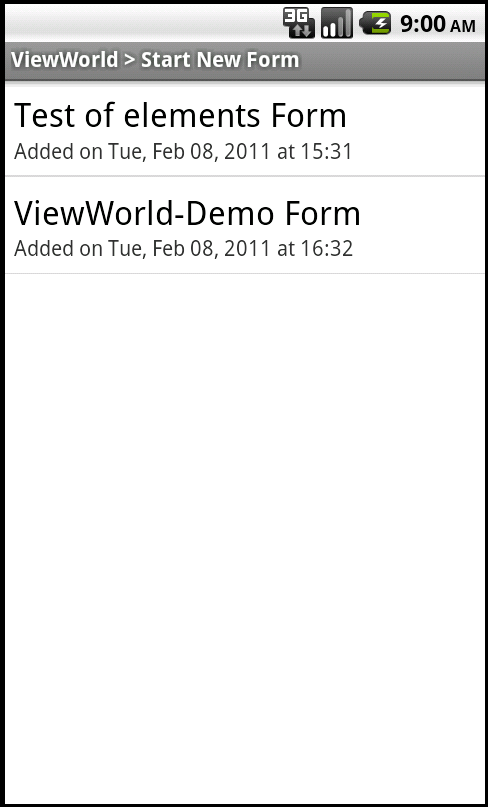
\includegraphics[width=0.35\textwidth]{pics/start_new_form_list.png}
  \caption{The list shows the forms available for reporting}
  \label{fig:start_new_form_list}
\end{figure}

\begin{figure}[H]
  \centering
      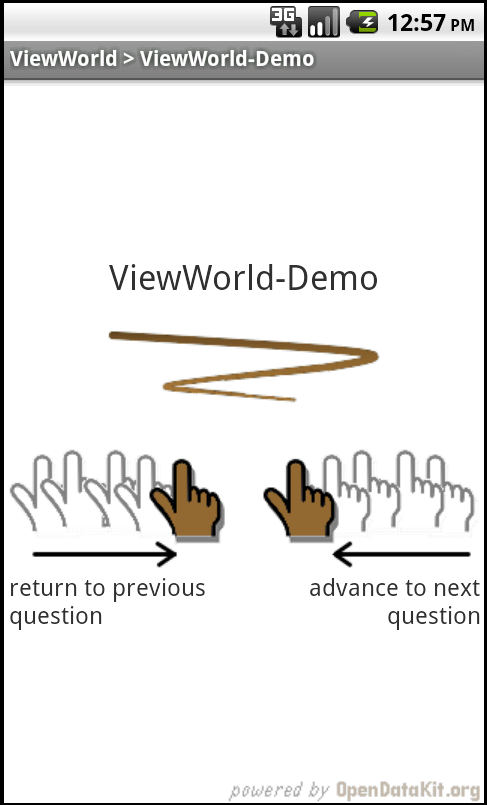
\includegraphics[width=0.35\textwidth]{pics/new_report_first_screen.png}
  \caption{Move between the different questions by sliding a finger across the screen}
  \label{fig:new_report_first_screen}
\end{figure}

When sliding your finger to the left, the first question appear. An example of a question can be seen in figure \ref{fig:new_report_picture}. In this case it is a picture that must be taken. The questions include entering text, numbers, recording GPS coordinates, images and selecting from a list of options.

When you have completed all questions you will arrive at the last screen of the report. This can be seen in figure \ref{fig:new_report_finished}. This page lets you save the report so it can be sent at a later time when internet access is available. On the last screen you should mark \emph{Mark Data as Finished} before clicking on \emph{Save Data And Exit}.
When you have saved data you are ready to start a new report or send data to the server.

\vspace{0.5cm}
\begin{boxedminipage}{\textwidth}
\textbf{IMPORTANT:}\\When recording GPS coordinates it takes up to 2 minutes to get a sattelite fix. Make sure that you are in an area with clear view of the sky. Close to trees and buildings it can be difficult to get a GPS fix.
\end{boxedminipage}

\begin{figure}[H]
  \centering
      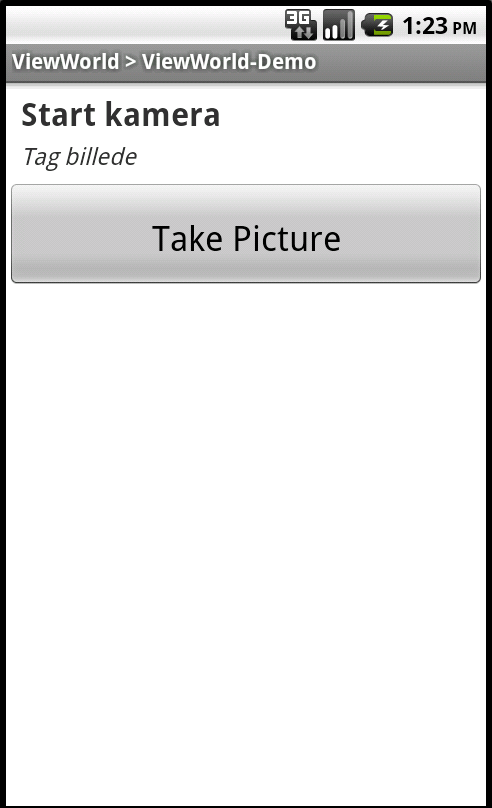
\includegraphics[width=0.35\textwidth]{pics/new_report_picture.png}
  \caption{This report contains a picture and lets you take a picture by pressing \emph{Take Picture}}
  \label{fig:new_report_picture}
\end{figure}

\begin{figure}[H]
  \centering
      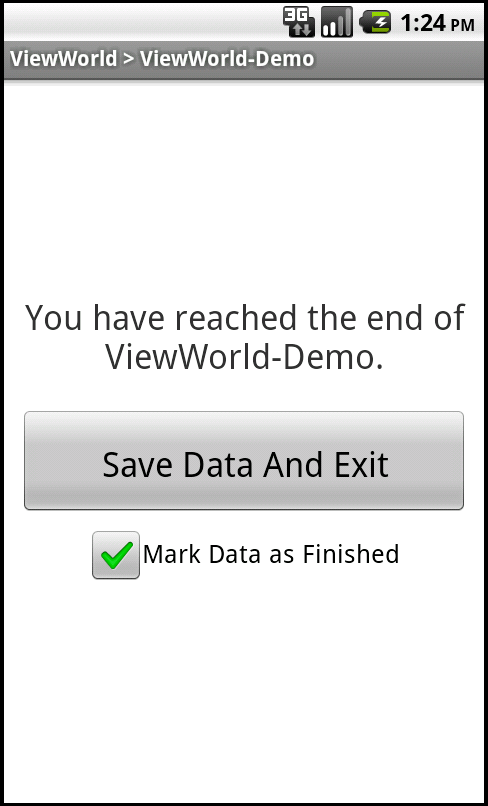
\includegraphics[width=0.35\textwidth]{pics/new_report_finished.png}
  \caption{The last question in a report lets you save the data on the phone. Remember to select \emph{Mark Data as Finished}}
  \label{fig:new_report_finished}
\end{figure}

\subsubsection{Sending reports}

To send reports to the server you press the \emph{Send Finished Data} in the main menu. This shows a list of all finished reports which are ready to be sent to the server as seen in figure \ref{fig:send_finished_data}. Only reports which have been marked \emph{Mark Data as Finished} when being saved will show up in this list.

Mark all the reports you wish to send to the server by pressing the checkmark to the right of the report. You can also mark all reports for sending by pressing the \emph{Toggle All} button.

When you have marked the reports you wish to send press the \emph{Send Selected} button and wait until you get the message \emph{Item(s) sent successfully}. You have now sent the report to the server, and the report dissapear from the finished report list.

\begin{figure}[H]
  \centering
      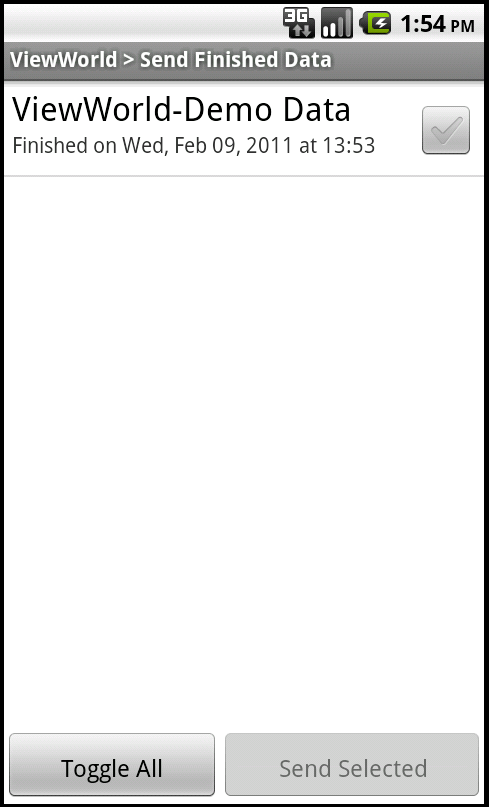
\includegraphics[width=0.35\textwidth]{pics/send_finished_data.png}
  \caption{List showing all finished data ready to be sent to the server. Mark what you wish to send and press \emph{Send Selected}}
  \label{fig:send_finished_data}
\end{figure}

\vspace{0.5cm}
\begin{boxedminipage}{\textwidth}
\textbf{IMPORTANT:}\\It may take a long time to upload data on a slow mobile network if images or videos have been recorded. Consider whether the connection is fast enough in the field, or whether you want to wait until the data can be uploaded via a WiFi connection.
\end{boxedminipage}

\subsection{Advanced use}
This part of the user manual is not described yet. Please feel free to provide input to the manual to Rune Persson on \url{rbp@viewworld.dk}.


\section{Web-interface}

The ViewWorld web interface allows you to access all data which has been reported using the ViewWorld android app. The data is available in a list and map view, and allows viewing, editing, deleting and exporting the reported data. 

\subsection{Login to web-interface}

To login to the web-interface you require a login user name and password from your organisation. Please contact your organisation for the details, as ViewWorld do not distribute passwords directly.

Login to the system by using your browser, and type in \url{viewworld.dk/login} in the address field. 

\vspace{0.5cm}
\begin{boxedminipage}{\textwidth}
\textbf{IMPORTANT:}\\The ViewWorld web interface does not support internet explorer 7, Firefox 3.5, Apple safari 3 or older browsers. Please update your browser if you use one of these. The Google Chrome browser is recommended for use with ViewWorld.\end{boxedminipage}

\subsection{View report data}

To view the collected data, login to the system as discribed above.

In the top left corner select the form name of the reports you wish to view. When clicking on the button a list as seen in figure \ref{fig:web_select_report}.

\begin{figure}[H]
  \centering
      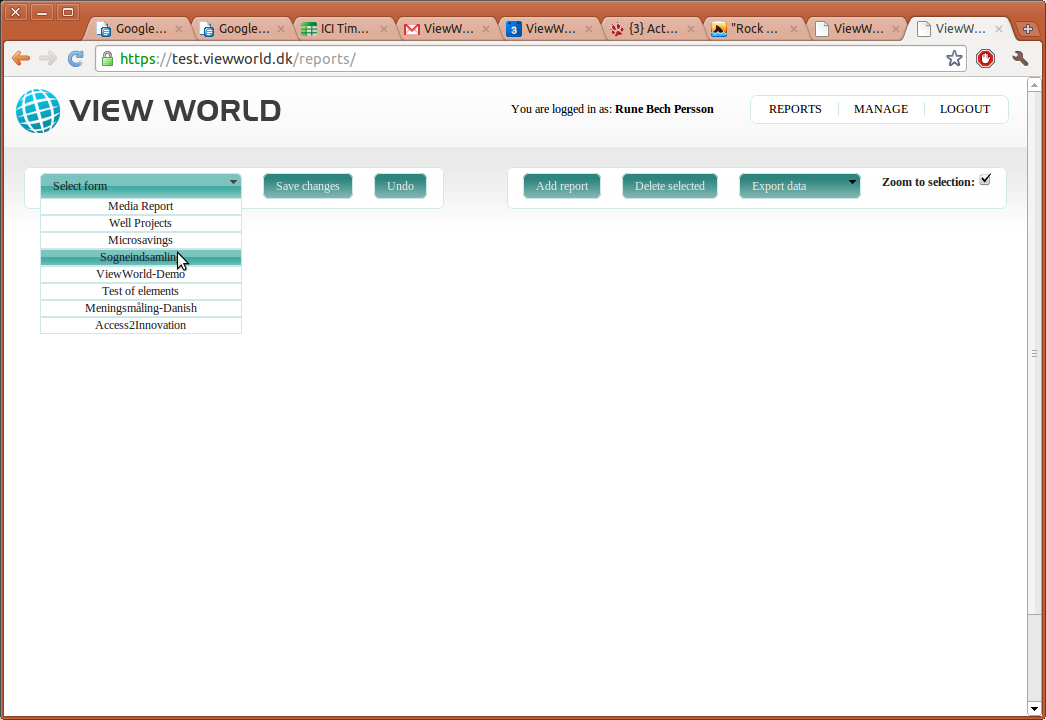
\includegraphics[width=0.9\textwidth]{pics/web_select_report.png}
  \caption{Select the form name of the reports you wish to view from the list}
  \label{fig:web_select_report}
\end{figure}

Only forms which you are authorized to view will appear in the list. When you have selected a form, the data for the form is displayed in a list view as seen in figure \ref{fig:web_view_demo_data}

\begin{figure}[H]
  \centering
      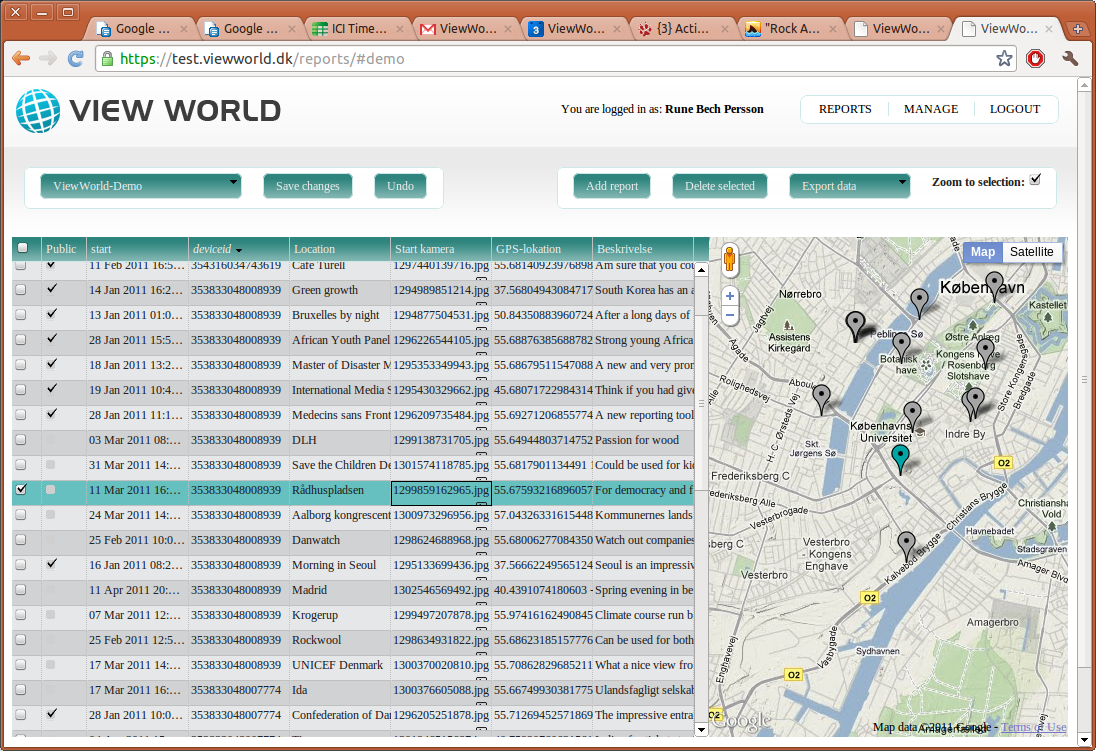
\includegraphics[width=0.9\textwidth]{pics/web_view_demo_data.png}
  \caption{View of collected data in a list and map}
  \label{fig:web_view_demo_data}
\end{figure}

Each row in the list is one report sent from the phone. The reports arrive in the list view shortly after they are sent from the phone, and the list view will continue to grow as more and more reports have been sent. 

When clicking on a report it is highlighted with a green color, and the map in the right side shows the location where the report was made with a green marker as seen in figure \ref{fig:web_view_demo_data}. The view automatically zooms in on the selected report in the map. If the map should not zoom in when a report is selected, you can unmark the \emph{Zoom to selection} in the top right corner of the page.

\subsubsection{Ordering report data}

By clicking on the title of a coloumn, the reports can be ordered. If clicking on a coloumn containing numbers, the list is sorted by increasing numbers, when clicking on a text coloumn, it is sorted alphabetically. Sorting works for dates, numbers, text, select one and multiple select questions.

In the example in figure \ref{fig:web_view_demo_data} the list is sorted by \emph{deviceid}.

\subsubsection{View media data}

Viewing media data is done by double clicking on a media element. At present, only pictures can be viewed directly in the web interface, where other types of media files such as videos and sound recordings will have to be downloaded to be playes.

To view an image in a report, double click on the image, and the image will be shown as in figure \ref{fig:web_view_picture}.

\begin{figure}[H]
  \centering
  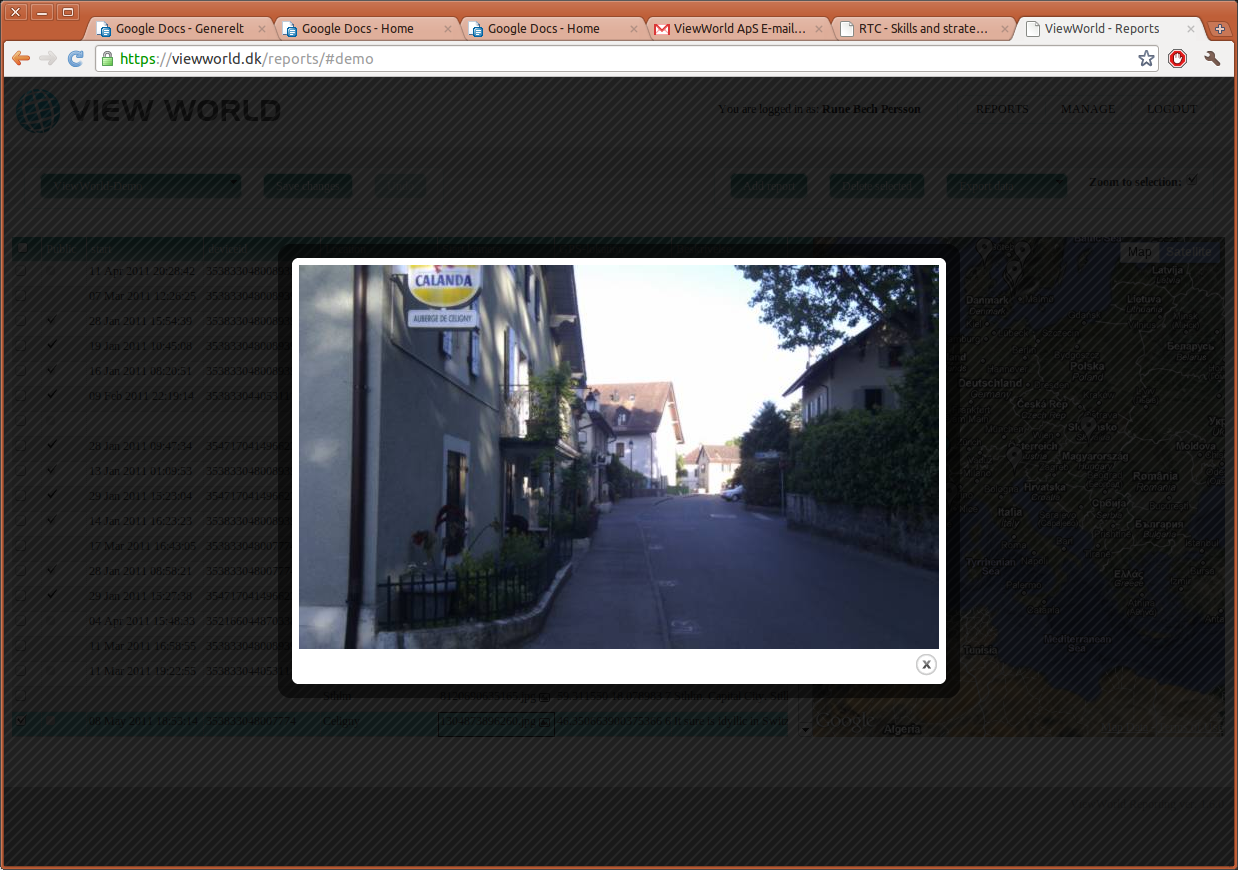
\includegraphics[width=0.9\textwidth]{pics/web_view_picture.png}
  \caption{View a picture from a report by double clicking}
  \label{fig:web_view_picture}
\end{figure}

Clicking on other types of media data, will download the media file. A player capable of playing the media file will have to be installed. The free player vlc is recommended, and can be downloaded from \url{http://www.videolan.org/vlc/}

\subsection{Edit report data}

Editing an element is easy. Simply double click on an element, sets the system into an edit mode. There are different editors based on the type of the element.
Two examples of editing a selection question and a date question can be seen in figure \ref{fig:web_edit_date} and \ref{fig:web_edit_select_one}.

\begin{figure}[H]
  \centering
  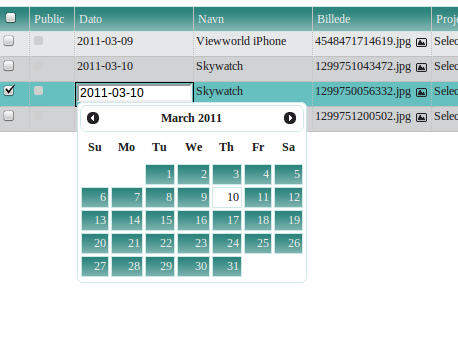
\includegraphics[width=0.6\textwidth]{pics/web_edit_date.png}
  \caption{Edit a date element by double clicking}
  \label{fig:web_edit_date}
\end{figure}

\begin{figure}[H]
  \centering
  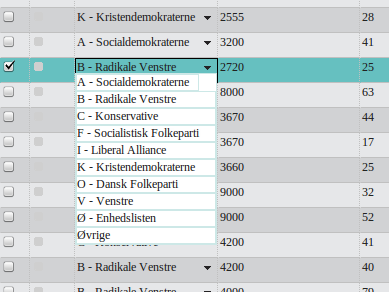
\includegraphics[width=0.6\textwidth]{pics/web_edit_select_one.png}
  \caption{Edit a selection element by double clicking}
  \label{fig:web_edit_select_one}
\end{figure}


When an element has been edited, you still have the ability to undo the changes. Do this by pressing the undo button. Each time the undo button is pressed, a change is undone. To save data to the database, click on the \emph{Save changes} button. 

The edit buttons available are described below:

\begin{description}
\item[Save changes] Saves the changes which have been made in the report data. Before saving the data, no change has been made on the server. When pressing \emph{Save changes} the changes are saved and cannot be un-done.
\item[Undo] Undo unsaved changes which have been made to the report data.
\item[Add report] Add a new report to the top of the list. The new report is empty, but can be filled in by using the web-interface. Some elements cannot be filled in when using the web-interface, which currently includes gps-coordinates, start-time, and all media data.
\item[Delete selected] Deletes one or several reports. This function should be used with care, as no undo function exists once a report has been deleted. 
\end{description}

\subsection{Export data}

Data can be exported from the system by clicking on the export data button in the top view.

All data for the selected form can be exported as a .csv or .pdf file. The .csv file is comma seperated, and can be imported in eg. excel for further calulations on data. The pdf file shows all report data in a list form.

\subsection{Managing users}

A management interface for super users allows creation of organisational users. However for the normal user, only changing of password is allowed.

To change your password, click on the management button in the top of the screen in the reports view. An option for changing password appear. Please note that the new password must be at least 6 characters long.

\vspace{0.5cm}
\begin{boxedminipage}{\textwidth}
\textbf{IMPORTANT:}\\If you have lost your password, please send an email to info@viewworld.dk with your name and organisation and we will send you a new temporary password. You must change the temporary password to your own password as soon as possible.\end{boxedminipage}


\section{Troubleshooting}

This part of the user manual is not described yet. Please feel free to provide input to the manual to Rune Persson on \url{rbp@viewworld.dk}.



\end{document}